% -*- latex -*-
%-----------------------------------------------------------------------
%;  Copyright (C) 1999
%;  Associated Universities, Inc. Washington DC, USA.
%;
%;  This program is free software; you can redistribute it and/or
%;  modify it under the terms of the GNU General Public License as
%;  published by the Free Software Foundation; either version 2 of
%;  the License, or (at your option) any later version.
%;
%;  This program is distributed in the hope that it will be useful,
%;  but WITHOUT ANY WARRANTY; without even the implied warranty of
%;  MERCHANTABILITY or FITNESS FOR A PARTICULAR PURPOSE.  See the
%;  GNU General Public License for more details.
%;
%;  You should have received a copy of the GNU General Public
%;  License along with this program; if not, write to the Free
%;  Software Foundation, Inc., 675 Massachusetts Ave, Cambridge,
%;  MA 02139, USA.
%;
%;  Correspondence concerning AIPS should be addressed as follows:
%;          Internet email: aipsmail@nrao.edu.
%;          Postal address: AIPS Project Office
%;                          National Radio Astronomy Observatory
%;                          520 Edgemont Road
%;                          Charlottesville, VA 22903-2475 USA
%-----------------------------------------------------------------------
%Body of AIPSletter for 15 October 1999

\documentclass[twoside]{article}
\usepackage{graphics}

\newcommand{\AIPRELEASE}{October 15, 1999}
\newcommand{\AIPVOLUME}{Volume XIX}
\newcommand{\AIPNUMBER}{Number 2}
\newcommand{\RELEASENAME}{{\tt 15OCT99}}
\newcommand{\OLDNAME}{{\tt 15APR99}}
\newcommand{\NEXTNAME}{{\tt 31DEC99}}

%macros and title page format for the \AIPS\ letter.
\input LET98.MAC
%\input psfig

\newcommand{\MYSpace}{-11pt}

\normalstyle

\section{General developments in \AIPS}

\subsection{Current and future releases}

The \AIPRELEASE\ release of Classic \AIPS\ is now available.  It may
be obtained via \emph{anonymous} ftp or by contacting Ernie Allen at
the address given in the masthead.  \RELEASENAME\ is also available
on CDrom as well as the more traditional tape media.  \AIPS\ is now
copyright \copyright\ 1995 through 1999 by Associated Universities,
Inc., NRAO's parent corporation, but may be made freely available
under the terms of the Free Software Foundation's General Public
License (GPL)\@.  This means that User Agreements are no longer
required, that \AIPS\ may be obtained via anonymous ftp without
contacting NRAO, and that the software may be redistributed (and/or
modified), under certain conditions.  The full text of the GPL can be
found in the \texttt{15JUL95} \Aipsletter.  A convenient order form is
found from our Web page at {\tt http://www.cv.nrao.edu/aips}.  A paper
order form and the ftp address appear on the last page of this
\Aipsletter.

We do not intend to have any further formal releases.  Instead, the
next ``release'' of \AIPS\ is called \NEXTNAME\ and is already
available via the Internet.  We will continue to correct and improve
\AIPS\ in this ``\AIPS\ for the Ages'' version indefinitely.  You may
fetch and install a complete copy of this version at any time.  Having
done so, you may update your installation whenever you want either as
a whole or by running the so-called ``midnight job'' which uses
transaction files to copy and compile the code selectively based on
the code changes and compilations we have done.  See articles later in
this \Aipsletter\ for details of this change in procedure and for
information on new tools to make such installations very much easier
to do.  Note that the midnight job allows your site to receive the
latest improvements and bug fixes, at the cost of also receiving the
latest bugs.  The latter can and will be fixed as rapidly as possible
when the programmers are notified of them at \texttt{daip@nrao.edu}.

\subsection{Highlights}

The \AIPRELEASE\ version contains only three new tasks and as many new
pseudoverbs.  Of these, the most significant is {\tt SETFC} which
prepares field description cards for input to {\tt IMAGR} including
outlier fields taken from a summary of strong sources in the NVSS, a
copy of which is now provided with \AIPS\@.  {\tt IMAGR} itself was
changed to allow up to 512 fields, to allow very large shifts, to do
the SDI Clean method optionally, and to filter away weak, isolated
Clean components.  {\tt CLIPM} is a version of {\tt CLIP} for
multi-source files and {\tt EXTAB} replaces {\tt TAPQL} for preparing
contents of \AIPS\ tables for use in spread sheets and the like.
Print routines, run interactively, can now adjust themselves to the
width of the user's display window.  Significant bugs related to {\tt
FITAB}, {\tt UVCOP}, {\tt IMAGR}, and {\tt CLIP} were corrected and
released as patches to {\tt 15APR99}\@.

\eject

\section{Improvements of interest to users in \RELEASENAME}

\emph{The {\tt 15APR98} release introduced numerous changes which are
not compatible with previous releases.  Disk files written by previous
versions are read transparently by {\tt 15APR98} and later releases
(including {\tt SAVE}/{\tt GET} files), but users must not attempt to
read disk files written by any of the modern versions with earlier
versions.  {\tt 15APR98} and later {\tt AIPS} cannot start previous
versions of tasks and the TV displays of the versions are
incompatible.  The TV displays of {\tt 15OCT98} and {\tt 15APR98} are
also not fully compatible.  {\tt SAVE}/{\tt GET} files for {\tt
15OCT98} and later releases cannot be read by {\tt 15APR98} and
earlier releases; {\tt 15OCT98} and later releases will translate old
{\tt SAVE}/{\tt GET} files when they encounter them.  Releases prior
to {\tt 15OCT98} are not fully Y2k compliant.}

\subsection{Imaging}

\subsubsection{SETFC}

The new task {\tt SETFC} has been written to prepare field-descriptor
cards for input to {\tt IMAGR} in its {\tt BOXFILE} option.  The work
on this task was begun by T. Joseph W. Lazio (NRL) and continued by
Bryan Butler (NRAO) before being completed by the \AIPS\ group.  The
task first prepares a list of fields to sample fully the center of the
region toward which the array was pointed.  Then, optionally, it
searches the NVSS (21-cm NRAO VLA Sky Survey) catalog for strong
sources near the pointing position and puts fields on them.  Finally,
if the Sun is near the pointing position, it puts a field on it.  User
adverbs control the size of the fields, the degree of overlap, and the
definitions of ``strong'' and ``near.''  The NVSS catalog is provided
in a minimal form (only the coordinates and the flux) in text files
supplied with the \AIPS\ release.  The full NVSS catalog and image
data base may be accessed through {\tt
http://www.cv.nrao.edu/\home{jcondon}/nvss.html}.

\subsubsection{IMAGR}

The Steer-Dewdney-Ito (SDI) flavor of the Clean algorithm is designed
to handle extended objects.  At some stage in every deep Clean, the
residual image will have had all small-diameter objects removed and
will effectively contain only extended areas of emission.  An option
to switch from the familiar Clark-Cotton-Schwab Clean to the SDI Clean
at this point has been added to {\tt IMAGR}\@.  It is triggered by a
user parameter specifying how negligible the high-flux tail of the
histogram of the residual must be to use SDI rather than BGC Clean.
The task can actually switch back and forth between the two methods.
Rather than taking a single component at the peak of the residual
image, the SDI method takes components at all pixels in the residual
image having flux above some current level.  If the same gain is
applied to all such components, the residual image after they are
subtracted will have bright rims around each extended region since
less flux is subtracted at the edges than is subtracted when all
adjacent pixels have components.  \AIPS\ task {\tt SDCLN} uses a
rather expensive algorithm to adjust the gains of the components to
try to avoid this problem.  {\tt IMAGR}'s algorithm is much faster but
less effective.  Nonetheless, the SDI method does help avoid the
corrugations which standard Cleans add to extended sources.

Clean has been found to remove flux from real sources and to place it
instead in pixels selected by noise bumps and sidelobes.  The task
{\tt CCSEL} was devised to eliminate weak, isolated Clean components
from a {\tt CC} file.  An improved version of this algorithm has now
been added to {\tt IMAGR}\@.  Clean components which have flux less
than a user-specified amount within a user-specified radius are
removed from the {\tt CC} files before the Clean components are
restored to the output images.  The filtering action may also be
selected from the TV menu during the Clean, when it will likely be
more useful.

{\tt IMAGR} and all tasks which accept image Clean components as models
can now handle up to 512 fields.  The various field-specifying adverbs
({\tt FLDSIZE}, {\tt RASHIFT}, {\tt BCOMP}, etc.) retain the old
dimension of 64.  You must use the {\tt BOXFILE} option to specify
these adverbs to {\tt IMAGR}\@.  A new kind of card has been added to
this option so that all of the {\tt BCOMP}s may be specified.  At the
same time, the meaning of {\tt RASHIFT}, {\tt DECSHIFT}, and {\tt
SHIFT} was changed for {\tt IMAGR} and many other tasks.  These are no
longer shifts in arc seconds in the {\tt -SIN} projection.  Instead
they are ``simple'' shifts in the {\tt -GLS} projection:
\begin{eqnarray*}
  \mbox{{\tt RASHIFT}} & = & (\alpha - \alpha_0) * \cos (\delta_0) \\
  \mbox{{\tt DECSHIFT}} & = & \delta - \delta_0
\end{eqnarray*}
This new convention allows for the very large shifts required at low
frequency to which the {\tt -SIN} projection cannot be applied.
(Users of large projections will of course set {\tt DO3DIMAG} to true
when using {\tt IMAGR}\@.)  All tasks were also corrected at this time
to recognize the {\tt -NCP} projection used by East-West
interferometers and to do the correct phase shifts for this
projection.

Lesser changes to {\tt IMAGR} included:
\begin{itemize}
\item\ {\tt IMAGR} now deletes its work file on exiting unless one of
       {\tt IN2NAME}, {\tt  IN2CLASS}, or {\tt IN2SEQ} are set.  The
       work file is sometimes useful for finding bad data through
       excessive residuals seen in various $uv$ printing and plotting
       tasks.
\item\ The methods by which {\tt IMAGR} selects the next field to
       Clean in {\tt OVERLAP 2} mode were improved and a bug that
       caused it to re-select fields that had just been done was
       corrected.
\item\ A TV option to override {\tt IMAGR}'s selection of the next
       field to Clean was added.  You may specify the next field and
       have it recomputed rather than having to force all fields to be
       recomputed.  This option is available when the number of fields
       is $> 64$ or when the user specifies {\tt DOWAIT} true before
       starting {\tt IMAGR}\@.
\item\ Two bugs in the data weighting routine were corrected.  In one,
       microscopic differences in round off could cause it to seek
       incorrect rows and get into all sorts of trouble.  In the
       other, the absence of data near $|u| \approx 0$ could cause
       memory addressing problems and incorrect results.
\end{itemize}

\subsection{Data display}

\begin{description}
\myitem{PLOTR} is a new task designed to read a text file containing
               plot labels and $x-y$ data and make an \AIPS-standard
               plot file.  Up to 5 different data types each with its
               own symbol may be plotted.
\myitem{DOCRT} was changed in all printing tasks and verbs to request
               the actual width of the terminal window so long as
               $0 <$ {\tt DOCRT} $ \leq 72$.  Larger values of {\tt
               DOCRT} are used without regard for the window width as
               before.
\myitem{FUNCTYPE}\hspace{0.5cm} {\tt = 'SQ'} for a square-root
               transfer function was added to all TV displays using
               this adverb.  It is often a good compromise between
               linear and logarithmic transfer functions, showing both
               low and high levels.
\myitem{LWPLA} was changed to allow multiple plot files to be written
               in a single job to the printer or a saved output file.
               Plots may be added to the latter in later jobs.  Such
               multi-page plot files are then not encapsulated and may
               have to be broken apart if you need to include them in
               a paper.
\myitem{SNPLT} was changed to plot dispersive delay.  It was then
               substantially rewritten.  It can now plot multiple
               polarizations and/or IFs and is able to plot them
               separately or plot both polarizations and/or all IFs on
               single plots (per antenna).
\myitem{POSSM} was corrected to plot small time averages efficiently.
               Previously, when {\tt SOLINT} was specified, the task
               could spend vast amounts of time looking at and
               calibrating data it did not need.  Problems caused by
               the first plot on a page having no data were corrected.
\myitem{UVHGM} had the {\tt PIXRANGE} adverb added.
\end{description}

\subsection{General and miscellaneous matters}

\subsubsection{New task to export table data}

It is sometimes useful to be able to analyze \AIPS\ table data outside
\AIPS\@.  The new task {\tt EXTAB} will write \AIPS\ table data to a
simple text file that can easily read by other programs such as
spreadsheets, database programs, and data analysis programs like
IDL\@.  You may select specific rows and columns to be exported in
the same way as you select rows and columns to be printed in {\tt
PRTAB}\@.   The task {\tt TAPQL} was deleted; it exported data for a
specific database format which is no longer used.

\subsubsection{New pseudoverbs}

Three new pseudoverbs were written to help users manipulate the
task-specific adverbs.  If you enter {\tt DEFAULT} followed by a task
name, the adverb values for that task alone are changed to the values
they would have on a full initialization ({\tt RESTORE 0}) without
changing any other adverb values.  Prior to {\tt 15OCT98}, adverb
values were stored only in a single {\tt TPUT}/{\tt TGET} files and
were over-written on any {\tt TPUT} or {\tt GO} for that task.  These
files function as always in the new release, but users may set up
parallel {\tt VPUT}/{\tt VGET} files specified by adverb {\tt VNUMBER}
from 1 through 35 for their own use in storing and retrieving adverb
values in a task-specific way.  No special meaning is attached to any
of these files by \AIPS, although some canned procedures may (in
future) use one or more of them.  {\tt GO} does not write into these
files; otherwise their use is the same as {\tt TPUT} and {\tt TGET}.
The new verb {\tt VGINDEX} will list the contents of the specified
{\tt VPUT}/{\tt VGET} file.

\subsubsection{Tape problems}

The relatively new task {\tt FITAB} was found to have several errors
and a rather complex ``gotcha.''  If a $uv$ file was written by {\tt
FITAB}, then read back in and modified in some way (\eg\ {\tt UVCOP}),
and then written out by {\tt FITTP}, the output would not be read
correctly thereafter.  The problem arose from a liberal use of \AIPS\
history cards in {\tt FITAB} and the retention of these histories by
the FITS readers.  After the correction, old \AIPS\ history cards are
no longer written by {\tt FITTP} and {\tt FITAB}\@.  Before the
correction, {\tt FITAB} had no problems because it wrote the current
information after the history file, but {\tt FITTP} had to write the
current file descriptors before the history, thereby confusing the
FITS readers.  If you have files which may have this problem, try
setting the new {\tt ERROR} adverb in the FITS readers ({\tt UVLOD},
{\tt IMLOD}, {\tt FITLD}) to 2 after encountering a problem reading
the file with {\tt ERROR} set at any other value.  This bypasses the
history parsing to avoid the bug.

Two serious errors caused the output of {\tt FITAB} to be useless
under different conditions.  Quantized images did not have meaningful
data written.  Tables with no time column were written with no data
when a $uv$ file was being written out in multiple pieces.  Both of
these errors crept in after most of the testing due to ``simple''
fixes.  {\tt FITAB} now writes the coordinates in both an \AIPS-normal
fashion and in the new proposed FITS keywords for tables extensions.

\subsubsection{Single dish}

{\tt OTFUV} was found to have an internal limit to the number of
channels.  It was changed to use the global {\tt MAXCHA} and {\tt
MAXCHA} was changed to 16384, the same as {\tt MAXCIF} which is the
product of channels, IFs, and polarizations.  The single-dish data
translation and indexing routines were fixed to run correctly on
byte-swapped computers.  The tasks used for beam-switched imaging were
enhanced.  {\tt BSGRD} now allows two different convolution functions
for the two convolutions it has to do (to azimuth-elevation and then
to RA-Dec) and it corrects for a rotation in the switch direction with
a shift rather than a rotation (which was a wrong thing to do).  A new
modeling task {\tt BSMOD} was installed to generate totally artificial
data to test various aspects of this observing mode.  A poster was
presented at ADASS IX on the subject by Eric Greisen.  The four-page
paper may be accessed at
{\tt ftp://ftp.cv.nrao.edu/egreisen/SWpaper.ps.gz} and the poster at
{\tt ftp://ftp.cv.nrao.edu/egreisen/SWposter.my.ps.gz}.  Pat Smiley
did a nicer version of the poster but it is a large file found at
{\tt ftp://ftp.cv.nrao.edu/egreisen/PatPost.eps.gz}.


\subsubsection{Miscellaneous}

\begin{description}
\myitem{CCEDT} had its {\tt CPARM}s reordered and changed to allow
        circular as well as rectangular apertures.  It was corrected
        to handle {\tt CC} tables with 7 as well as 3 columns.  It now
        uses image increment based tolerances and defaults and uses
        dynamic memory so that it can try to handle any size of
        problem.
\myitem{XTRAN} was changed to do only its ``plate-solution'' mode.
        There are several better tasks for re-gridding image
        geometries.  An option to copy the image and alter only the
        output header was added to avoid any re-gridding.  Finally
        serious errors in the re-gridding and in the handling of
        sub-images were corrected.  This task is still not correct for
        large images, but it now works very much better for smaller
        ones.
\myitem{ORDER} is a new adverb to specify the order of a polynomial
        fit.  It is used by {\tt FLGIT}, {\tt UVLSF}, {\tt UVLIN},
        {\tt IMLIN}, and other tasks.  The first 3 of these were
        changed to allow 0-order as well as first-order fits.
\myitem{IMEAN} was changed to be able to write the actual rms and mean
        into the image header under control of the adverb {\tt
        DOCAT}\@.  The {\tt ACTNOISE}  header parameter is used by
        {\tt SAD}, {\tt IMFIT}, and {\tt JMFIT} in evaluating the
        errors in their Gaussian fits.
\myitem{IRING} was changed to take {\tt APARM} as relative to the
        reference pixel rather than the ``center'' of the current
        sub-image.
\myitem{COMB} had a bug handling blanked pixels in the {\tt MEAN}
        operation corrected.
\end{description}

\subsection{VLBI data processing}

\subsubsection{FITLD}

The handling of VLBA weights in {\tt FITLD} has been improved. The
weights assigned to VLBA data are now proportional to their
integration time so that data from baselines using shorter
integrations are not weighted too highly relative to those from
baselines using longer integration times.

\subsubsection{Miscellaneous changes}

\begin{description}
\myitem{CVEL} now supports the {\tt QUAL} adverb to improve the
              selection of which sources are shifted.
\myitem{PCCOR} allows selection of IFs for the case when two separate
              bands are observed simultaneously.  Selection of good
              data was improved.
\myitem{ANTAB} was modified to attempt to cope with Tsys measurements
              made by non-NRAO telescopes between scans.  The adverb
              {\tt OFFSET} was added to allow the user to specify the
              amount of time that should be added to both ends of a
              scan to include the Tsys measurements in the apparent
              scan range.
\myitem{COHER} was given the option to solve for a variable coherence
              time as a function of baseline and time.  The output is
              in a format suitable for direct input to {\tt BLING}\@.
              This option is likely to be particularly relevant at
              millimeter wavelengths.
\myitem{CL2HF} was modified at GSFC  by Dave Gordon and the
              modifications installed in the official release.  Good
              results have been reported.
\end{description}

\subsubsection{Fringe fitting}

This release fixes a number of errors associated with the exhaustive
baseline search option of {\tt FRING} which is controlled by {\tt
DOFIT} and {\tt APARM(9)}\@.  These errors caused the least-squares
routines to be called with faulty starting estimates for the delays
and rates with the result that the exhaustive baseline search would
sometimes fail to find fringes that would have been found in the
default mode or would sometimes arrive at an incorrect delay and rate.

Some errors in the allocation of array processor memory that caused
{\tt FRING} to claim that it was out of memory when channels were
selected using {\tt BCHAN} and {\tt ECHAN} have also been fixed in
this release.

The least-squares stage of {\tt KRING} has now been completely
replaced.  This was necessary for reworking the SNR calculation to use
the same methods as found in the FFT\@.  For test data, the two stages
now produce SNRs that agree to within 1\%.  Many inputs were removed
from {\tt KRING} including the ability to create/fill an output file
for single source data.  Since {\tt KRING} requires an {\tt NX} table,
this was disallowed anyway.  Averaging the frequencies within an IF is
not allowed anymore either; {\tt KRING}'s more efficient use of memory
renders this sort of option unnecessary.  The default SNR cutoff
threshold has been lowered to 3.  The help file has been updated
somewhat but likely still needs some user input.  The output format
has been cleaned up as well to be more readable and the print levels
consolidated.

\subsection{Interferometric data handling}

\subsubsection{Data modeling}

When {\tt CC} files are used as a source model, the model computations
may be controlled with {\tt NCOMP}\@.  A previously undocumented
feature of this was the ability to cut off the computation at the
first negative in each {\tt CC} file if any of the {\tt NCOMP} was
specified as a negative number.  This feature has now been documented
and a new, scientifically correct, cut off method has been added.  The
adverb {\tt FLUX} was added to all such tasks to specify the minimum
absolute value of the component flux to be used in modeling.

\subsubsection{Editing}

A new task called {\tt CLIPM} was written to edit multi-source files.
It writes entries in the flag table based on amplitudes out of range
for observations selected and calibrated with all of the usual
(numerous) adverbs.  For spectral-line data, it works hard to keep the
number of flags minimal.  Nonetheless, a great many may be created.
{\tt UVCOP} is able to apply up to 50000 flags to a single time which
allows users to avoid the 5000 limit in the rest of \AIPS\@.  An
option to flag all channels if $\ge n$ are clipped was added to both
{\tt CLIPM} and the older {\tt CLIP} used on single-source files.  An
error handling compressed data from the VLBA correlator was corrected
in {\tt CLIP}\@.

The interactive editing tasks {\tt EDITA}, {\tt EDITR} and {\tt SNEDT}
received some attention.  The adverb {\tt EXPERT} was added to
instruct these tasks to begin in ``expert'' (keyboard input) rather
than menu (mouse input) mode.  Bugs applying current flags to data in
the one antenna at a time mode, in getting the correct value of
{\tt DOTWO} in {\tt TY} editing, in recognizing the new {\tt FLAG
QUICKLY} function, and in flagging the first point in that mode were
corrected.  The method used to handle times was revised; the old
method should have failed frequently but only did so on Linux systems.
The defaults for {\tt SOLINT} and {\tt DETIME} were changed to plot
every point.

\subsubsection{Ugly error in UVCOP}

{\tt UVCOP} set a mask to select the desired spectral channels and
IFs.  Unfortunately, it used the increments in the output data set
rather than the input data set.  If the frequency axis precedes the IF
axis, data selection errors occurred if both {\tt BIF} $ > 1$ and {\tt
BCHAN}/{\tt ECHAN} selected fewer than all of the spectral channels.
The error appeared in {\tt 15OCT98} on August 24, 1998 when a line of
code a long ways away was changed to correct another problem and that
changed variables in a {\tt COMMON}\@.  We can hope that people do not
normally sub-select both IFs and channels at the same time.

\subsubsection{Miscellaneous corrections and additions}

\begin{description}
\myitem{CALIB} has a new adverb {\tt ANTUSE} to control which antennas
               are used in the calculation of the mean gain modulus.
               An error applying an Lpol-only model to data with all
               polarizations was corrected.
\myitem{QUACK} has a new option to flag data at the end of each scan.
               The handling of times was corrected and some control
               given to the user for data with short integration
               times.
\myitem{SPLAT} and {\tt UVAVG} had their handling of random parameters
               generalized to handle all current ones and to do
               something reasonable with future ones.  An unnecessary
               operation was removed from {\tt SPLAT} and the program
               now runs very much faster when averaging.
\myitem{LDGPS} and {\tt APGPS} continued to be developed and tested.
               They load GPS data to a {\tt GP} table and then use the
               GPS delay data to calculate phase corrections due to
               the excess path length of the ionosphere and to
               calculate the ionospheric Faraday rotation.
\end{description}

\vfill\eject
\section{Matters of interest to programmers and \AIPS\ Managers}

\subsection{Support for the Intel Platform Edition of Solaris}

The {\tt 15OCT99} release of \AIPS\ includes support for the Intel
Platform Edition of Solaris.  This is the version of Solaris that is
used on PC-compatible computers.  Sun have made both the Intel
platform and the SPARC platform editions of Solaris available to
non-commercial users for the cost of media, shipping and handling. See
{\tt http://www.sun.com/developers/tools/solaris/solarispromo.html}
for details on this offer.

There are no precompiled \AIPS\ binaries for this platform so you will
have to build \AIPS\ from the sources using {\tt INSTEP2} and {\tt
INSTEP4}. The default configuration assumes that you are using the GNU
Compiler Collection.  Prebuilt versions of the GNU Compiler Collection
(as well as other useful tools) are available at {\tt
http://www.sunfreeware.com} for both SPARC and Intel.

As is the case with the SPARC Platform Edition of Solaris, the Intel
Platform Edition is not optimally configured to run \AIPS\ efficiently
as shipped. Some hints on tuning Solaris for \AIPS\ are available at
{\tt http://www.aoc.nrao.edu/~cflatter/solaris-.html}.

\subsection{Problems with GNU FORTRAN Under Solaris}

We have recently uncovered a fault in the Solaris implementation
of the standard C library that gives rise to a minor problem in
versions of \AIPS\ that have been compiled using GNU FORTRAN 77 under
Solaris. If you append output text to an existing file in programs
that have an {\tt OUTFILE}-like adverb, then you will lose some of the
data in that file. There is no problem if you always specify a new
output file so few \AIPS\ users are likely to be inconvenienced by
this problem.

We are still investigating this problem and will publish any further
information to the {\tt alt.sci.astro.aips} newsgroup and the {\tt
bananas} mailing list as it becomes available.  This problem is known
to occur under all versions of Solaris from 2.5.1 onwards (both
platform editions) but does not occur if you are using the Sun
compilers.

\subsection{Brief items}

\begin{description}
\myitem{AIPSEXEC} \hspace{1cm} now allows the user to specify the
           debugger (\eg\ {\tt debug=dbx}) on the {\tt aips} command
           line.  If {\tt AIPS} itself is to be debugged, the command
           becomes, for example, {\tt debug=gdb:aips}.  The prompt for
           debugger name failed occasionally under Linux.
\myitem{NETSP} warnings for disks not defined have been restricted to
           the {\tt AIPS} program itself.
\myitem{MNJ} Midnight jobs will henceforth be required to use the
           secure shell ({\tt ssh}).  The methods used previously
           lacked security and would not be able to expand to meet the
           expected increase in demand.
\myitem{FSTVS3} is a variable in the {\tt DSEL.INC} calibration
           commons that was not used seriously before.  It is now a
           counter of the true visibility record number.  A new
           subroutine {\tt FINDUV} uses this variable to find the next
           desired time interval in a data set and the corresponding
           range of visibility numbers.
\end{description}

\section{AIPS for the Ages}

The {\tt 15OCT99} release of Classic \AIPS\ will be the last formal
release of \AIPS\@.  The current distribution model for \AIPS\ of
periodic releases continues to serve the community well.  However,
faced with declining \AIPS\ staffing levels, we feel it is necessary
to reduce the amount of system work and concentrate on application
programming and bug-fixes.  The final ``release'' of \AIPS\ will be
{\tt 31DEC99}, the so-called ``\AIPS\ for the Ages'' (\AIPS\ for the
Aged?).  This version is already available, for complete download or
for incremental updates, from the \AIPS\ Web page.  Bug-fixes and new
tasks will implemented in {\tt 31DEC99} (and the \Aipsletter\ will
continue to appear approximately every six months) until the NRAO user
community completes the transition to the recently-released \AIPTOO\@.

\eject

\section{Installing Aips for the Ages}

We are intending to make the installation and updating of {\tt
31DEC99} as painless as possible.  As we see it, there are four
categories of installation situations:
\begin{enumerate}
\item\ installing {\tt 31DEC99} as the site's first \AIPS\
          installation,
\item\ installing {\tt 31DEC99} for the first time, but the site has
          earlier \AIPS\ version(s) installed,
\item\ installing all of {\tt 31DEC99} over the top of an old
          installation of {\tt 31DEC99}, and
\item\ installing any updated pieces of {\tt 31DEC99} over the top of
          a relatively current copy of {\tt 31DEC99}\@.
\end{enumerate}

In the first 3 categories, the \AIPS\ Manager begins by obtaining a
copy of {\tt 31DEC99.tar.gz} via our Web pages.  This Gnu-zipped
``tarball'' is created every night and contains a current copy of all
\AIPS\ source code and documentation.  It is currently 31 Mbytes in
size and can usually be copied over the Internet in a reasonable time.
The on-line \AIPS\ Order Form will eventually provide a way to order
{\tt 31DEC99} on CDrom.

{\it At present,} the Manager in category 1 has to install \AIPS\ in
the usual sequence of steps.  This involves downloading and unpacking
the tarball, running the {\tt INSTEP1} script, optionally downloading
binaries from Charlottesville or compiling them locally, and setting
up and initializing the \AIPS\ control files using {\tt FILAIP}, {\tt
POPSGN}, and {\tt SYSETUP}.  All of this is well documented in the
installation summary ({\tt http://www.cv.nrao.edu/aips/install.ps}).
{\it In the future,} a new {\tt install.pl} perl script will permit a
much easier installation process.  Watch the \AIPS\ Web site for an
announcement of this script.

The Manager faced with category 2 or 3 problems can already use a new
and tested perl script called {\tt update.pl}.  Category 3 is really
category 2 except for a first step of renaming the old {\tt 31DEC99}
directory tree to something else before creating the new one.
Category 4 is particularly simple.  The installation procedures now
create (or will when category 1 is upgraded) files needed to run what
is known as the ``midnight job'' (MNJ, so named as it should be run
between midnight and 8 a.m. US/Eastern time).  This ``job'' detects
changes to the \AIPS\ transaction files in Charlottesville, and then
performs any needed operations for the local site.  This may include
copying modified files from Charlottesville, compiling subroutines,
and linking tasks.  The job ends by generating a nice report which
shows what it did and all new entries in {\tt CHANGE.DOC} made by the
\AIPS\ Group.  This midnight job is usually run as a {\tt cron} job at
a regular time every day, week, or month.  In addition or instead, it
can be run manually whenever the Manager decides to do so.

The above-mentioned {\tt update.pl} script for a category 2/3 update
greatly simplifies the process.  The Manager (1) gets the tarball and
puts it in the {\tt \$AIPS\_ROOT} area, and then (2) copies {\tt
update.pl} to disk, makes it executable, and runs it.  {\tt update.pl}
won't (yet) run {\tt INSTEP2} or {\tt INSTEP4} or {\tt POPSGN} for
you, but it does just about everything else,  Anything left over is
summarized for you in a checklist that is printed out when the script
ends.  This will be a {\it very small\/} subset of the work \AIPS\
Managers had to contend with in previous updates.  The first line of
{\tt update.pl} will need to be edited if perl is not located at {\tt
/usr/local/bin/perl}.  The script requires perl version 5 or better.

{\tt update.pl} runs {\tt MAKE.MNJ} to prepare for later use of the
midnight job.  Sites with ``legacy'' entries in the master {\tt
UPDCONFIG} file should delete the {\tt \$SYSLOCAL/UPDCONFIG} that {\tt
MAKE.MNJ} now creates; new MNJ sites will use this local file.

The requirements for the new midnight job are:
\begin{itemize}
\item\  A moderately recent version of the {\tt ssh} client is
    available on your system (\eg\ 1.2.25).
\item\ You have already set up a key for the account which will run
    the \AIPS\ midnight job by running the {\tt ssh-keygen} program.
\item\ You chose {\tt \$HOME/.ssh/} as a location for the keys when
           you ran {\tt ssh-keygen} (this is the default).
\item\ You {\it only} want to use the secure version of the MNJ for
           your primary access to {\tt mnj.cv.nrao.edu}.
\item\ You have gotten the ``MNJ'' private key (a binary file) from
           Pat Murphy, preferably via secure mail (PGP preferred; his
           public key is available on the web at\\ \hspace*{1.4cm}{\tt
           http://www.cv.nrao.edu/\home{pmurphy}/plan.html}).\\
           Place the MNJ file in  the {\tt \$HOME/.ssh/} directory,
           and {\tt chmod} it to mode 0600.
\item\ You have set up a {\tt do\_daily.{\it xxxx}} script to run your
    MNJ on computer {\it xxxx}.  If you plan to run it via {\tt cron},
    make sure the script sets {\tt \$PATH} enough that {\tt ssh} and
    other basic utilities are found.  A sample {\tt do\_daily} script
    is given below.
\item\ You are not running the ssh-agent program; if the variable
    {\tt SSH\_AGENT\_PID} is {\it not} set, then you can proceed to
    the next step.  You can check if it's set by typing the command:
    {\tt echo \$SSH\_AGENT\_PID}\@.  If this command only shows a
    blank line, you are not running an agent. If it shows a number
    like 20415, you are.  If you are, you {\it must} first invoke the
    command: {\tt ssh-add -D} before proceeding to the next step.
    This command temporarily deletes all identities from your agent.
    You can add them back after the next step; it's only necessary
    when first setting up the MNJ (or if running the job by hand when
    you have an agent running; ssh likes to use your main identity
    even when told to use the MNJ one).
\item\ ``Prime'' the system by giving the command:\\\hspace*{1.4cm}
    {\tt ssh mnj.cv.nrao.edu -i .ssh/mnj -l aipsmgr
    /AIPS/31DEC99/COPYING}\\ (do this from your home directory, or
    alter the path to the {\tt .ssh/} directory) and answer ``yes''
    when it asks if you want to add {\tt mnj.cv.nrao.edu} to the list
    of known hosts.  If this command is  successful, it will print out
    a copy of the \AIPS\ General Public License (The ``GNU GPL'')\@.
    Once you have verified this ssh command works, you can add back
    any identities to your agent if you deleted them.
\item\ Run your {\tt do\_daily.{\it xxxx}} script interactively, check
    the logs, look for the output from {\tt AIPSUPD} in the log that
    says {\tt AIPSUPD - Using the SECURE SHELL for copying}.  If there
    are no other obvious errors (and files were really copied!) then
    you're ready to run the MNJ whenever you want.  Otherwise you may
    need to contact Pat Murphy for assistance.
\end{itemize}

A site may run more than one midnight job.  In that case, typically,
the site will have only one copy of the \AIPS\ source code and one
computer will run a ``primary'' MNJ to Charlottesville.  After that
has run, other computer architectures may run ``secondary'' MNJs using
NFS access to the single copy of the source code and running only the
compilation and link edit parts of the transactions.  In this way, a
site's storage of \AIPS\ is kept simple by having a single copy
serving more than one architecture and the load on the Charlottesville
computers is kept to a minimum.  Converting secondary MNJ jobs to use
the secure shell can be tricky; contact Pat Murphy if you really want
to do this.  The following is a sample {\tt do\_daily.{\it xxxx}}:
\begin{center}
\begin{verbatim}
          #!/bin/sh
          #                                   fix path for cron, etc.
          ######################## Change for local account names/files
          [ "$HOME" = "" ] && HOME=/home/jenlan/egreisen
          . $HOME/.profile.path
          ########################
          # following assumes "something.hostname" as name of file
          myname=`basename $0 | awk -F. '{print $2}'`
          [ "`uname -n | awk -F. '{print $1}'`" = "$myname" ] || exit
          #                                   set AIPS logicals
          ######################## Change for local $AIPS_ROOT
          cd /home/analysis/aips
          ########################
          . ./LOGIN.SH
          $CDTST >/dev/null 2>&1
          #                                   remove any old binaries
          (cd $LOAD; find . -name '*.EXE.OLD' -atime +2 -exec rm -f {} \;)
          #                                   Go to MNJ area
          cd $AIPS_VERSION/$ARCH/UPDATE
          #                                   Now do the MNJ
          ./AIPSUPD TST
\end{verbatim}
\end{center}
\vfill\eject

\section{Patch Distribution}

As before, important bug fixes and selected improvements in
\RELEASENAME\ can be downloaded via the Web at:

\begin{center}
\vskip -10pt
{\tt http://www.cv.nrao.edu/aips/15APR99/patches.html}
\vskip -10pt
\end{center}

Alternatively one can use {\it anonymous} \ftp\ on the NRAO cpu {\tt
aips.nrao.edu}.  Documentation about patches to a release is placed
in the anonymous-ftp area {\tt pub/aips/}{\it release-name} and the
code is placed in suitable subdirectories below this. Information on
patches and how to fetch and apply them is also available through the
World-Wide Web pages for \hbox{\AIPS}.  As bugs in \RELEASENAME\ are
found, the patches will be placed in the {\tt ftp}/Web area for
\hbox{{\RELEASENAME}}.  No matter when you receive your \RELEASENAME\
``tape,'' {\it you must} fetch and install these patches if you
require them.

The \OLDNAME\ release had a number of important patches announced.
These were:
\begin{enumerate}
\item\ {\tt TVCPS} and other tasks that use the image catalog
       (1999-05-14, 1999-06-18).
\item\ {\tt APGPS} and {\tt TECOR} (delay calibration modes) (1999-05-14).
\item\ {\tt CLIP}, {\tt RESEQ}, {\tt DTCHK} problems with compressed
       data (1999-05-25).
\item\ {\tt REGRD} crashed under Solaris, others (1999-07-06).
\item\ {\tt UVCOP} errors selecting channels (1999-07-21).
\item\ {\tt IMAGR} in {\tt OVERLAP 2} mode selects wrong fields
       (1999-07-22).
\item\ {\tt FITAB} followed by {\tt FITTP} makes unreadable files
       (1999-07-27).
\item\ {\tt FITAB} did not write image tables and quantized floating
       images (1999-08-09).
\item\ {\tt PRTTP} patched code did not convert {\tt DOCRT} to
       reasonable values (1999-09-07).
\end{enumerate}

\section{Progress on a world-coordinates standard}

At the ADASS meeting held in Boston in the Fall of 1992 it was decided
that a standard for conveying coordinate information within the FITS
format needed to be developed.  Eric Greisen was, in his absence,
volunteered for the effort.  Versions of possible standards authored
by Greisen and Mark Calabretta (of the ATNF in Australia) began
appearing in June 1993 and have appeared at irregular intervals since.
At the 1999 ADASS meeting held in Kona Hawaii, Eric and Mark were
instructed to make a few minor corrections to the current drafts of
the papers and then to submit them for formal review by the U.S.,
European, and Japanese FITS Committees.  The paper is now divided into
three parts: a general paper, a celestial-coordinates paper, and a
spectral-coordinates paper.  All three of these are available via the
WWW and we encourage you to fetch and read them.  When these are
adopted --- and something very much like them will become part of the
FITS standard --- they will affect the ways in which we think about
astronomical data.  For that reason alone, they are important and we
solicit your comments ({\tt egreisen@nrao.edu} and {\tt
mcalabre@atnf.csiro.au}).  The papers are:
\renewcommand{\labelenumi}{\Roman{enumi}.}
\begin{enumerate}
\item\  Representations of world coordinates in FITS, by Greisen and
  Calabretta\\
  ({\tt ftp://ftp.cv.nrao.edu/NRAO-staff/egreisen/wcs.ps.gz})
\item\ Representations of celestial coordinates in FITS, by Calabretta
  and Greisen\\
  ({\tt ftp://ftp.cv.nrao.edu/NRAO-staff/egreisen/ccs.ps.gz})
\item\ Representations of spectral coordinates in FITS, by Greisen\\
  ({\tt ftp://ftp.cv.nrao.edu/NRAO-staff/egreisen/scs.ps.gz})
\end{enumerate}
\renewcommand{\labelenumi}{\arabic{enumi}.}
The 1999 ADASS poster on WCS is also available as a
\begin{itemize}
\item\  4-page summary ({\tt
   ftp://ftp.cv.nrao.edu/NRAO-staff/egreisen/Paper99.ps.gz})
\item\ poster ({\tt
   ftp://ftp.cv.nrao.edu/NRAO-staff/egreisen/Poster99.ps.gz})
\end{itemize}
\vfill\eject

\section{\AIPS\ Distribution}

The total distribution of the {\tt 15OCT98} release was under-reported
in the last \Aipsletter\ due to a glitch in accessing log files
following an upgrade to our FTP server.  Instead of 263 copies, we
actually distributed 321.  The \AIPS\ distribution history over the
last few years is plotted in the accompanying figure (prepared with
the new {\tt PLOTM} task) and shows a gratifying and continued
increase over the last year and a half.  This increase probable
reflects both the new capabilities in \AIPS\ and the improvements in
the installation process.

\centerline{\resizebox{!}{3.0in}{\includegraphics{15OCT99.plt}}}

A total of 361 copies of the {\tt 15APR99} release were distributed to
344 non-NRAO sites.  Of these, 187 were in source code form and 174
were distributed as binary executables. The figures on computers using
\AIPS\ are affected by the percentage of \AIPS\ users that register
with NRAO\@.  Of 344 non-NRAO sites receiving {\tt 15APR99} only 85
(25\%) have registered.  We remind serious \AIPS\ users that
registration is required in order to receive user support.  The first
table below shows the breakdown of how the copies of {\tt 15APR99}
were distributed and includes both source-code distributions and
binary distributions.  The second table below is based on the
disappointing number of registered installations of {\tt 15APR99}\@.
It lists total numbers of computers and indicates that the
distribution over operating systems was heavily weighted toward
Solaris with Linux as a distant second.  However, when asked about
``primary'' architecture, 46\%\ of our users answered Linux and 40\%\
answered some flavor of Sun OS\@.  This indicates how far Linux has
penetrated as the system used on the more powerful computers used by
astronomers today.  The third table gives information about the
geographic distribution of the systems shipped.

\begin{center}
\begin{tabular}{|l|r|r|r|r|r|r|} \hline\hline
              &{ftp} & {CDrom} &{8mm} & {4mm} & {ZIP} & {Floppy} \\ \hline
{\tt 15OCT98} & 242   &      71 &   8  &    1  &    0  &       0  \\ \hline
{\tt 15APR99} & 290   &      69 &   0  &    2  &    0  &       0  \\ \hline\hline
\end{tabular}
\end{center}

\begin{center}
\begin{tabular}{|l|r|r|r|r|r|r|r|} \hline\hline
{Operating System} & \texttt{15APR99} & \texttt{15APR99}  & \texttt{15OCT98}
                           & \texttt{15APR98}  & \texttt{15OCT97}
                           & \texttt{15APR97}  & \texttt{15OCT96} \\
                &  {No.}   & {\%} & {\%} & {\%} & {\%} & {\%} & {\%} \\
\hline
Solaris/SunOS 5 & 196 & 53 & 61 & 66 & 50 & 66 & 46  \\
PC Linux        &  99 & 27 & 27 & 19 & 23 & 16 & 19  \\
SGI             &  47 & 13 &  1 &  3 &  1 &  1 &  5  \\
Dec Alpha       &  14 &  4 &  3 &  7 &  9 &  6 & 10  \\
HP-UX           &   7 &  2 &  5 &  2 &  3 &  6 &  4  \\
SunOS 4         &   3 &  1 &  1 &  4 & 14 &  5 & 13  \\
IBM /AIX        &   1 &  0 &  2 &  1 &  0 &  0 &  4  \\
Alpha Linux     &   0 &  0 &  0 &    &    &    &     \\
Total           & 367 &    &    &    &    &    &     \\
\hline\hline
\end{tabular}
\end{center}

\begin{center}
\begin{tabular}{|llr|r|} \hline\hline
\multicolumn{3}{|c|}{ftp sites}&physical media sites \\
Domain & Location &                Number & Number  \\
\hline
ar  & Argentina                       & 1 &  4 \\
au  & Australia                       & 6 &    \\
be  & Belgium (Kingdom of)            & 1 &    \\
br  & Brazil  (Federative Republic of)& 1 &    \\
bg  & Bulgaria                        & 1 &  1 \\
ca  & Canada                         & 14 &  2 \\
com & U.S.A. (commercial)            & 29 &    \\
    & China                          &    &  3 \\
de  & Germany (Federal Republic of)  &  5 &  1 \\
edu & U.S.A. (education)             & 81 &    \\
es  & Spain (Kingdom of)             & 10 &    \\
fi  & Finland (Republic of)          &  3 &    \\
fr  & France (French Republic)       &  4 &    \\
gov & U.S.A. (government)            &  5 &    \\
gr  & Greece                         &  1 &    \\
hu  & Hungary                        &  1 &  1 \\
in  & India (Republic of)            &  3 &  2 \\
    & Israel                         &    &  1 \\
it  & Italy (Italian Republic)       &  6 &  2 \\
jp  & Japan                          & 20 &  1 \\
kr  & Korea (Republic of)            &  2 &  1 \\
mil & U.S.A. (military)              &  2 &    \\
mx  & Mexico (United Mexican States) &  3 &    \\
net & Network (largely U.S.A.)       & 42 &    \\
nl  & Netherlands                    &  7 &  1 \\
no  & Norway                         &  1 &    \\
pt  & Portugal                       &  2 &    \\
org & Organization (largely U.S.A.)  &  4 &    \\
ru  & Russia (Russian Federation)    &  2 &  1 \\
se  & Sweden (Kingdom of)            &  6 &    \\
tw  & Taiwan                         &  5 &    \\
    & United Arab Emirates           &    &  1 \\
uk  & United Kingdom (Great Britain) &  8 &  7 \\
us  & United States of America       &  1 & 36 \\
za  & South Africa                   &  1 &    \\
    & TOTAL                         & 278 & 65 \\
\multicolumn{4}{|c|}{Totals: USA=200, foreign=143} \\
\hline\hline
\end{tabular}
\end{center}

\section{\AIPS\ on CDrom}

Starting with {\tt 15APR98}, we have made \AIPS\ available on CDrom.
The initial tests using recordable CD's were very successful, and
resulted in a CD with source code, two binary versions (Linux and
Solaris), all {\tt DDT} files, and a GNU-zipped version of the
documentation ({\tt TEXT}) area.  It is possible to either perform a
full installation on disk (\ie\ copying the binaries from CD to local
disk), or to run from the \hbox{CD}.  In the latter case, the
``footprint'' on the local disk is under 10 Megabytes!  (This figure
does not include user data, obviously.)  Furthermore, the setup script
was given the ability to switch between a ``run from CD'' installation
and a ``full'' installation.  The fact that 69 copies of the {\tt
15APR99} CDrom were distributed suggests that this functionality, and
the availability of \AIPS\ on this new medium, are of considerable use
to the Astronomical Community.
\vfill
\eject

% Order form and mailer page
\cleardoublepage\pagestyle{empty}
\centerline{\resizebox{!}{23.3cm}{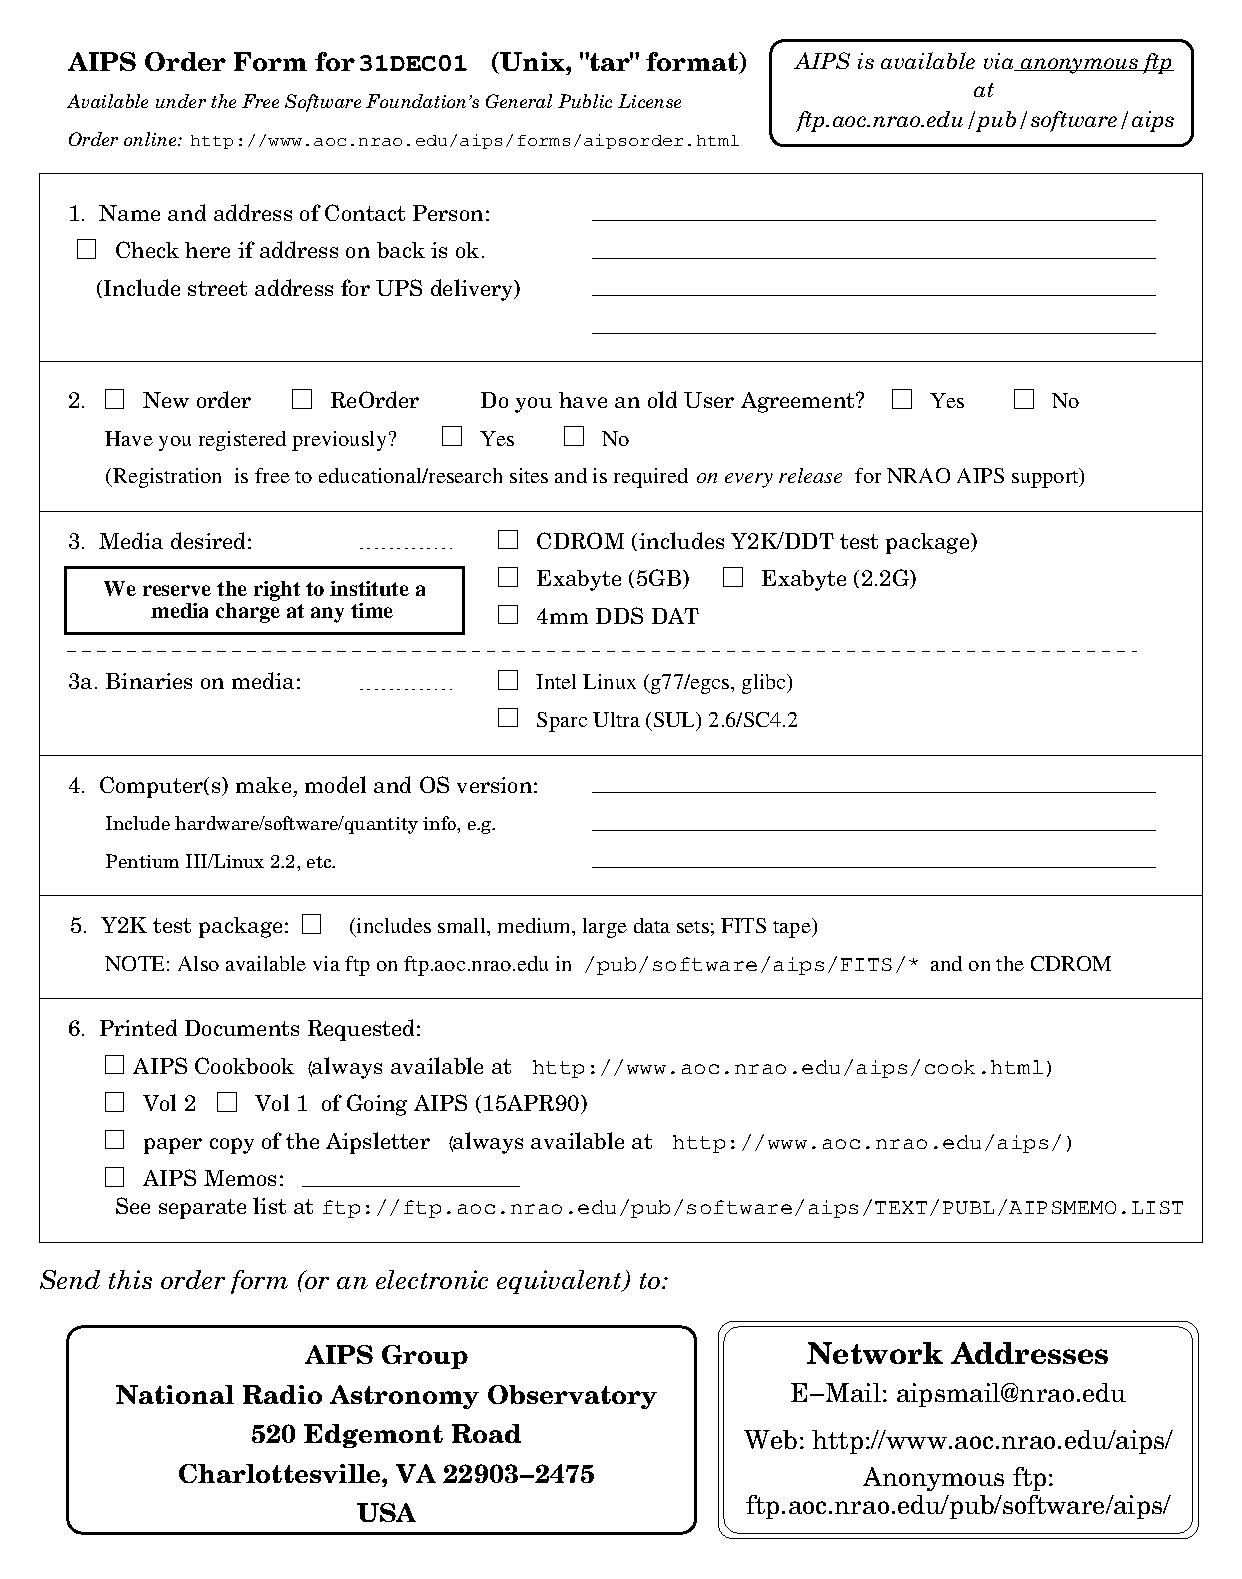
\includegraphics{FIG/AIPSORDER.PS}}}
 \vfill\eject
 \vbox to 4.4in{
  \vfill
  \centerline{\resizebox{!}{2.6in}{\includegraphics{FIG/Mandrill.eps}}}
  \vfill}
\phantom{...}
\centerline{\resizebox{!}{!}{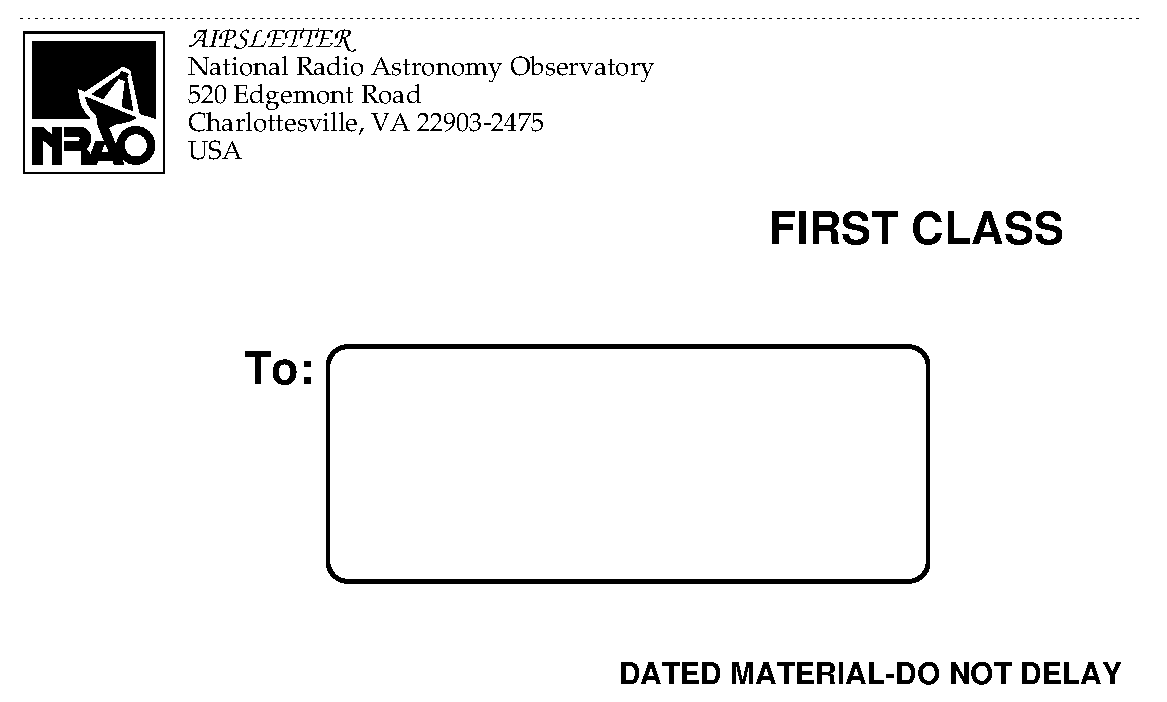
\includegraphics{FIG/AIPSLETM.PS}}}

\end{document}
